\label{sec:migration}
In a SDN virtualization infrastructure, the virtual networks are operated by installing flow rules in the underlying physical network.
In the event of a migration, for maintenance purposes or because of an attack, the flow rules will be redeployed on a different physical substrate.
Determining how the flow rules should be deployed and which physical nodes should be selected is called Virtual Network Embedding, and there already are various solutions doing so~\cite{Zangiabady2017e, Papagianni2013, Chowdhury2016d, Wang2015}.
We leave the VNE problem out of the scope of this thesis.
We also limit our study of migration process to the networking aspect of it, meaning that we are not considering the internal specificities of the hypervisors and how mappings between virtual and physical nodes are handled during the migration.
We study the flow rules that will be installed in the SDN nodes by the hypervisor because of the migration.

\begin{figure}[ht]
\centering
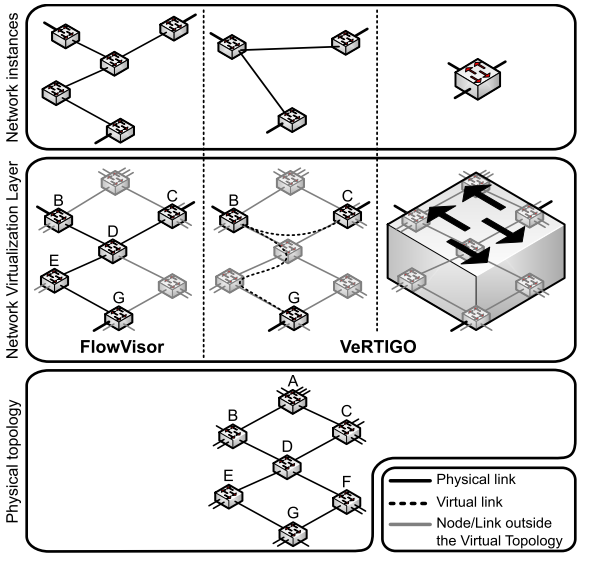
\includegraphics[scale=0.8]{figures/onetomany.png}
\caption{Example of 1-to-many mapping for virtual nodes and links, from VeRTIGO~\cite{VeRTIGO-Corin2012a}}
\label{fig:1tomany}
\end{figure}

We have presented in Section~\ref{sec:reference_archi} a reference architecture for the network hypervisor.
From the SDN point of view, a virtual link is a collection of flow rules deployed on one ore more physical node, to carry the traffic of a specific tenant.
Similarly, a virtual node is the end point of several flow rules.
Therefore, a virtual node can be seen a collection of flow rules describing the end point of several virtual links, SDN-wise.

We include in this work the possibility to describe a one-to-many mapping between a virtual node and a physical node.
Figure~\ref{fig:1tomany} (from VeRTIGO~\cite{VeRTIGO-Corin2012a}) depicts the one to many mapping between virtual and physical elements.

We describe two migration algorithms in the following subsections, a naive implementation and an more elaborate one.
These algorithms use different functions in order to migrate the topology: create\_link, delete\_link, create\_node, delete\_node and embedding. 
We explain what each function does, SDN-wise:

\begin{itemize}
\item Create\_link($vlink\_name,path$): This function will deploy flow rules related to $vlink\_name$ on the different nodes composing $path$. Returns the identifier of the migrated link.
\item Delete\_link($vlink\_name$): This function will remove the flow rules pertaining to $vlink\_name$ from the physical nodes embedding it.
\item Create\_node($vnode\_name,path$): This function will deploy flow rules related to $vnode\_name$ on the different nodes composing $path$. Returns the identifier of the migrated node.
\item Delete\_node($vnode\_name$): This function will remove the flow rules related to  $vnode\_name$ on the physical nodes embedding it.
\item embedding($vlink\_name|vnode\_name$) returns the physical substrate allocated by the VNE component for either $vlink\_name$ or $vnode\_name$.
\end{itemize}

\subsubsection{Move based Migration}
\label{sec:move-algo}

An intuitive migration algorithm is described in~\cite{Lime-Ghorbani2014}. 
This algorithm aims at migrating the resources all at once, as depicted in Algorithm~\ref{algo:move_algo}.
However, during the migration phase, the VNs are not operational as both are shutdown.
We propose our version of the algorithm (see Algorithm~\ref{algo:move_algo}) where during the migration phase, both VNs (old and new) will coexist.

First (line 3) we initialize $new\_topology$ as the migrated topology. Then, for each virtual node in the topology, we retrieve the new embedding decided by the VNE component (lines 4-5).
Then (line 6) we instantiate the new virtual node and add the information to $new\_topology$
We repeat the process for the virtual links (lines 7-9).
Then we remove the flow rules related to the old virtual nodes from the original substrate (lines 10-11) and from the old virtual links (lines 12-13).

An underlying aspect of the cohabitation of the old and new VNs is the necessity to redirect new incoming flows through the newly migrated VN.
This is handled by setting specific priorities for the flow rules corresponding to the VN.


\begin{algorithm}[ht]
\textbf{Input: }$topology$ as the virtual network\\
\textbf{Output: } $new\_topology$ as the migrated topology\\
% \State $nodes \gets List\_of\_nodes(topology)$
$new\_topology \gets \{\emptyset\}$\\
\For{$node$ \textbf{in} $topology$}{
$path \gets$ embedding($node$)\\
$new\_topology \gets$~$new\_topology$~$\cup$~create\_node($node$,$path$)
}
\For{$link$ \textbf{in} $topology$}{
$path \gets$ embedding($link$)\\
$new\_topology \gets$~$new\_topology$~$\cup$~create\_node($link$,$path$)
}
\For{$node$ \textbf{in} $topology$}{
delete\_node($node$)
}
\For{$link$ \textbf{in} $topology$}{
delete\_link($link$)
}
\caption{Move based algorithm}
\label{algo:move_algo}
\end{algorithm}


\subsubsection{Iterative Migration}
Another algorithm we consider is described in~\cite{vnm-lo2013}.
This algorithm iteratively moves nodes one after another, while dynamically creating links for the migrated nodes and deleting the old ones.
The migration progress is depicted in Algorithm~\ref{algo:iterative_algo}:
% Create two arrays, one to hold nodes left to be migrated, one to hold the nodes that have been migrated (lines 2-3).
Create a token to remember if this is the first iteration of the algorithm (Line 5).
% While there are nodes to be migrated, do the following (Lines 5 to 28):
Select a node among the remaining nodes (line 7), we refer to it as the old node, create the new node (line 9) and create the virtual links between the new node and the nodes that have not been migrated (lines 11-14).
If this is not the first iteration of the algorithm, there might be links to be established between the new node and the nodes that have already been migrated. (lines 15-20).
There may also be links between migrated nodes and the old node.
If so, they are deleted. (lines 21-24)



\begin{algorithm}[ht]
\textbf{Input: }$topology$ as the virtual network\\
\textbf{Output: } $new\_topology$ as the migrated topology\\
 $remaining\_nodes \gets list\_of\_nodes(topology)$\\
 $migrated\_nodes \gets \emptyset$\\
 $iter \gets 1$\\
\While {$remaining\_nodes \neq \emptyset$}{
 $n \gets Select\_node(remaining\_nodes)$\\
 $path \gets$ embedding($n$)\\
 $new\_n \gets$ create\_node($n,path$)\\
 \For{$node$ \textbf{in} $remaining\_nodes$}{
    \uIf{exist\_link($new\_n,node,topology$)}{
        $vlink \gets $link($new\_n,node,topology$)\\
        $path \gets$ embedding($vlink,topology$)\\
        create\_link($vlink,path$)\\
    }
 }
%  $Deploy\_links(new\_n,remaining\_nodes,topology)$\\
\uIf{$iter>1$}{
%  $Deploy\_links(new\_n,migrated\_nodes,topology)$\\
 \For{$node$ \textbf{in} $migrated\_nodes$}{
    \uIf{exist\_link($new\_n,node,topology$)}{
        $vlink \gets $link($new\_n,node,topology$)\\
        $path \gets$ embedding($vlink,topology$)\\
        create\_link($vlink,path$)\\
    }
 }
%  $Deleted\_links(n,migrated\_nodes,topology)$
 \For{$node$ \textbf{in} $migrated\_nodes$}{
    \uIf{exist\_link($new\_n,node,topology$)}{
        $vlink \gets $link($new\_n,node,topology$)\\
        delete\_link($vlink$)
    }
 }
 
 }
 $iter \gets iter + 1$\\
 $migrated\_nodes \gets migrated\_nodes \cup n$\\
 $remaining\_nodes \gets remaining\_nodes / \{n\}$\\
 $delete\_node(n)$\\
 }
\caption{Iterative migration algorithm}
\label{algo:iterative_algo}
\end{algorithm}


The following list details the functions used for the migration
%\GB{again, you are not providing an elaborate explanation with respect to the parameters.}.
%\FC{Done}
\begin{itemize}
\item $Select\_node$ selects the next node to be migrated.
\item exist\_link($node1,node2,topology$) returns True if there is a virtual link between $node1$ and $node2$ in $topology$.
\item link($node1,node2,topology$) returns the identifier of the virtual link connecting $node1$ and $node2$ in $topology$.
\end{itemize}